\documentclass{article}
\usepackage{tikz}
\usepackage{pgfplots}
\usepackage{amsmath}

\begin{document}

\begin{figure}[ht]
    \centering
    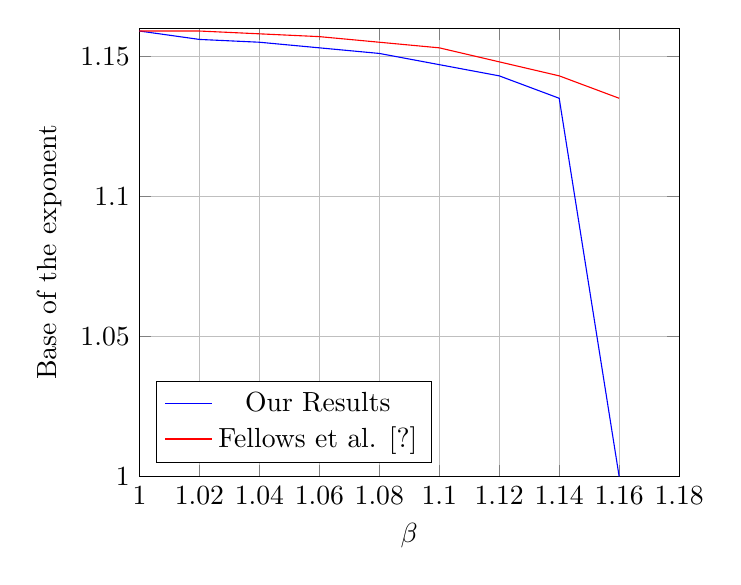
\begin{tikzpicture}
        \begin{axis}[xlabel={$\beta$},
                     ylabel={Base of the exponent},
                     xmin=1., xmax=1.18,
                     ymin=1., ymax=1.16,
                     xtick distance=.02,
                     ytick distance=.05,
                     grid=both,
                     legend pos=south west]
            \addplot+[no markers] coordinates {(1, 1.159) (1.02, 1.156) (1.04, 1.155) (1.06, 1.153) (1.08, 1.151) (1.1, 1.147) (1.12, 1.143) (1.14, 1.135) (1.16, 1.)};
            \addlegendentry{Our Results}
            \addplot+[no markers] coordinates {(1., 1.159) (1.02, 1.159) (1.04, 1.158) (1.06, 1.157) (1.08, 1.155) (1.1, 1.153) (1.12, 1.148) (1.14, 1.143) (1.16, 1.135)};
            \addlegendentry{Fellows et al. [?]}

        \end{axis}
    \end{tikzpicture}
\end{figure}

\end{document}